\chapter{Wstęp}
\section{Wprowadzenie}

Algorytmy automatycznej kontroli głośności(AGC) są ważnym elementem współczesnych systemów przetwarzania sygnałów audio. Zarówno do zastosowań telekomunikacyjnych, konferencyjnych jak i obróbki nagrań. Takie algorytmy mają na celu zapewnić stały poziom głośności mówców zarówno w czasie jak i między sobą.
Ważne jest aby takie algorytmy skutkowały wysokim poziomem sygnału do szumu(SNR) jak i wysokim stosunkiem sygnału do szumu do pozostałych interferencji- na przykład pogłosu.

Najprostszym rozwiązaniem jest zastosowanie prostego systemu jednokanałowego[JAKAŚ REFKA!]. W takim systemie możlie jest tylko sterowanie głośnością sygnału wejściowego, na podstawie chwilowej wartości obwiedni. Uniemożliwia on jednak różny poziom wzmocnienia dla różnych mówców i usunięcie interferencji.

Rozwiązaniem bardziej skomplikowanym, zarówno od strony sprzętowej, programistycznej i czasu obliczeń jest użycie systemu z wieloma mikrofonami. Taki system umożliwia pożądane rozróżnienie między mówcami i eliminację interferencji[REFKA!]. W systemie takim możliwa jest estymacja wektora sterującego, czyli kierunków nadchodzenia fali, a co za tym idzie mocy nadchodzącej z wybranych stron i zastosowanie odpowiednich filtrów, które wzmacniają sygnał z żądanych kierunków.

W tej pracy skupiono się właśnie na drugim z wymienionych rodzajów algorytmów AGC. W pracy zostanie przedstawiona praktyczna implementacja bazująca na nagraniach z macierzy mikrofonowych.

\begin{figure}[h]
    \centering
    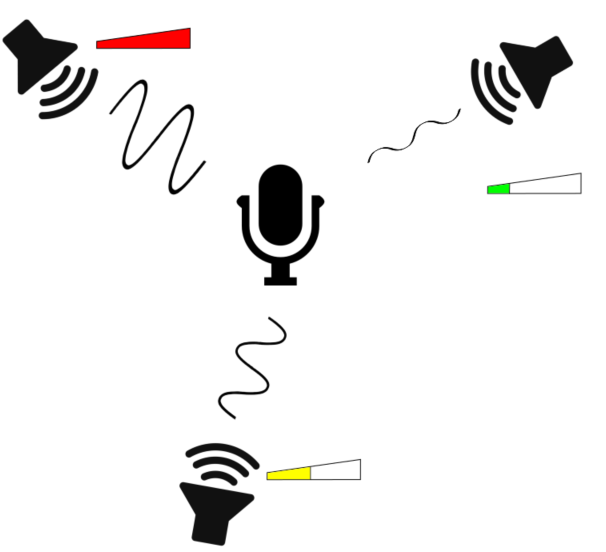
\includegraphics[width=\textwidth]{Images/setup.png}
    \caption{Graficzna reprezentacja problemu}
    \label{fig:setup}
\end{figure}

\section{Cel}
Celem pracy inżynierskiej była praktyczna implementacja istniejącego algorytmu AGC z tłumieniem tła akustycznego, wraz z estymacją kierunku nadchodzenia fali. Wybrany algorytm spełnia cechy wymienione w poprzedniej sekcji,tj. pozwala na regulację głośności nagrania zarówno w czasie jak i między mówcami i minimalizację zakłóceń. Jako zakłócenie do eliminacji przyjęto w niniejszej pracy biały szum gaussowski.

\section{Zakres wykonanej pracy}
Pierwszym z etapów pracy inżynierskiej było zapoznanie się autora pracy z dostępnymi publikacjami opisującymi zarówno tematykę AGC jak i generalną tematykę przetwarzania sygnałów dla macierzy czujników i wybór metody. 
Kolejnym etapem pracy. Następnie dokonany wyboru środowiska pracy- był to język Python. Szczegółowy opis użytych narzędzie znajduje się w [blablka]. Następnie autor pracy napisał symulator umożliwiający generację sygnałów mikrofonowych. Dalsza część realizacji pracy obejmowała- zaplanowanie praktycznej implementacji systemu, wykonanie tej implementacji i testy przy użyciu symulatora[tu wszędzie jaka sekcja itp].

